% Options for packages loaded elsewhere
\PassOptionsToPackage{unicode=true}{hyperref}
\PassOptionsToPackage{hyphens}{url}
%
\documentclass[
  12pt,
  oneside]{book}
\usepackage{lmodern}
\usepackage{amssymb,amsmath}
\usepackage{ifxetex,ifluatex}
\ifnum 0\ifxetex 1\fi\ifluatex 1\fi=0 % if pdftex
  \usepackage[T1]{fontenc}
  \usepackage[utf8]{inputenc}
  \usepackage{textcomp} % provides euro and other symbols
\else % if luatex or xelatex
  \usepackage{unicode-math}
  \defaultfontfeatures{Scale=MatchLowercase}
  \defaultfontfeatures[\rmfamily]{Ligatures=TeX,Scale=1}
\fi
% Use upquote if available, for straight quotes in verbatim environments
\IfFileExists{upquote.sty}{\usepackage{upquote}}{}
\IfFileExists{microtype.sty}{% use microtype if available
  \usepackage[]{microtype}
  \UseMicrotypeSet[protrusion]{basicmath} % disable protrusion for tt fonts
}{}
\makeatletter
\@ifundefined{KOMAClassName}{% if non-KOMA class
  \IfFileExists{parskip.sty}{%
    \usepackage{parskip}
  }{% else
    \setlength{\parindent}{0pt}
    \setlength{\parskip}{6pt plus 2pt minus 1pt}}
}{% if KOMA class
  \KOMAoptions{parskip=half}}
\makeatother
\usepackage{xcolor}
\IfFileExists{xurl.sty}{\usepackage{xurl}}{} % add URL line breaks if available
\IfFileExists{bookmark.sty}{\usepackage{bookmark}}{\usepackage{hyperref}}
\hypersetup{
  hidelinks,
}
\urlstyle{same} % disable monospaced font for URLs
\usepackage{color}
\usepackage{fancyvrb}
\newcommand{\VerbBar}{|}
\newcommand{\VERB}{\Verb[commandchars=\\\{\}]}
\DefineVerbatimEnvironment{Highlighting}{Verbatim}{commandchars=\\\{\}}
% Add ',fontsize=\small' for more characters per line
\usepackage{framed}
\definecolor{shadecolor}{RGB}{248,248,248}
\newenvironment{Shaded}{\begin{snugshade}}{\end{snugshade}}
\newcommand{\AlertTok}[1]{\textcolor[rgb]{0.94,0.16,0.16}{#1}}
\newcommand{\AnnotationTok}[1]{\textcolor[rgb]{0.56,0.35,0.01}{\textbf{\textit{#1}}}}
\newcommand{\AttributeTok}[1]{\textcolor[rgb]{0.77,0.63,0.00}{#1}}
\newcommand{\BaseNTok}[1]{\textcolor[rgb]{0.00,0.00,0.81}{#1}}
\newcommand{\BuiltInTok}[1]{#1}
\newcommand{\CharTok}[1]{\textcolor[rgb]{0.31,0.60,0.02}{#1}}
\newcommand{\CommentTok}[1]{\textcolor[rgb]{0.56,0.35,0.01}{\textit{#1}}}
\newcommand{\CommentVarTok}[1]{\textcolor[rgb]{0.56,0.35,0.01}{\textbf{\textit{#1}}}}
\newcommand{\ConstantTok}[1]{\textcolor[rgb]{0.00,0.00,0.00}{#1}}
\newcommand{\ControlFlowTok}[1]{\textcolor[rgb]{0.13,0.29,0.53}{\textbf{#1}}}
\newcommand{\DataTypeTok}[1]{\textcolor[rgb]{0.13,0.29,0.53}{#1}}
\newcommand{\DecValTok}[1]{\textcolor[rgb]{0.00,0.00,0.81}{#1}}
\newcommand{\DocumentationTok}[1]{\textcolor[rgb]{0.56,0.35,0.01}{\textbf{\textit{#1}}}}
\newcommand{\ErrorTok}[1]{\textcolor[rgb]{0.64,0.00,0.00}{\textbf{#1}}}
\newcommand{\ExtensionTok}[1]{#1}
\newcommand{\FloatTok}[1]{\textcolor[rgb]{0.00,0.00,0.81}{#1}}
\newcommand{\FunctionTok}[1]{\textcolor[rgb]{0.00,0.00,0.00}{#1}}
\newcommand{\ImportTok}[1]{#1}
\newcommand{\InformationTok}[1]{\textcolor[rgb]{0.56,0.35,0.01}{\textbf{\textit{#1}}}}
\newcommand{\KeywordTok}[1]{\textcolor[rgb]{0.13,0.29,0.53}{\textbf{#1}}}
\newcommand{\NormalTok}[1]{#1}
\newcommand{\OperatorTok}[1]{\textcolor[rgb]{0.81,0.36,0.00}{\textbf{#1}}}
\newcommand{\OtherTok}[1]{\textcolor[rgb]{0.56,0.35,0.01}{#1}}
\newcommand{\PreprocessorTok}[1]{\textcolor[rgb]{0.56,0.35,0.01}{\textit{#1}}}
\newcommand{\RegionMarkerTok}[1]{#1}
\newcommand{\SpecialCharTok}[1]{\textcolor[rgb]{0.00,0.00,0.00}{#1}}
\newcommand{\SpecialStringTok}[1]{\textcolor[rgb]{0.31,0.60,0.02}{#1}}
\newcommand{\StringTok}[1]{\textcolor[rgb]{0.31,0.60,0.02}{#1}}
\newcommand{\VariableTok}[1]{\textcolor[rgb]{0.00,0.00,0.00}{#1}}
\newcommand{\VerbatimStringTok}[1]{\textcolor[rgb]{0.31,0.60,0.02}{#1}}
\newcommand{\WarningTok}[1]{\textcolor[rgb]{0.56,0.35,0.01}{\textbf{\textit{#1}}}}
\usepackage{longtable,booktabs}
% Allow footnotes in longtable head/foot
\IfFileExists{footnotehyper.sty}{\usepackage{footnotehyper}}{\usepackage{footnote}}
\makesavenoteenv{longtable}
\usepackage{graphicx,grffile}
\makeatletter
\def\maxwidth{\ifdim\Gin@nat@width>\linewidth\linewidth\else\Gin@nat@width\fi}
\def\maxheight{\ifdim\Gin@nat@height>\textheight\textheight\else\Gin@nat@height\fi}
\makeatother
% Scale images if necessary, so that they will not overflow the page
% margins by default, and it is still possible to overwrite the defaults
% using explicit options in \includegraphics[width, height, ...]{}
\setkeys{Gin}{width=\maxwidth,height=\maxheight,keepaspectratio}
\setlength{\emergencystretch}{3em} % prevent overfull lines
\providecommand{\tightlist}{%
  \setlength{\itemsep}{0pt}\setlength{\parskip}{0pt}}
\setcounter{secnumdepth}{5}

% Set default figure placement to htbp
\makeatletter
\def\fps@figure{htbp}
\makeatother

%%%%%%%%%%%%%%%%%%%%%%%%%%%%%%%%%%%%%%%%%%%%%%%%%%%%%%%%%%%%%%%%%%%%%%%%%%%%%%%%
% University of Western Ontario Thesis Template
% 1. Initial version by: Justin Quinn Veenstra, 2010 with thanks to Mr. (soon to be Dr.) Will Robertson.
% 2. Adapted by: Dr. John Stuart Haberl Baxter, 2018 for his thesis.
% 3. Dr. Baxter's thesis converted to generic template by: Dr. Jonathan C. Lau, 2018.
% 4. Adapted for use with RMarkdown/Bookdown by: Thea Knowles (expected PhD 2019)

%%%%%%%%%%%%%%%%%%%%%%%%%%%%%%%%%%%%%%%%%%%%%%%%%%%%%%%%%%%%%%%%%%%%%%%%
%%                                                                    %%
%%                    ***   I M P O R T A N T   ***                   %%
%%                                                                    %%
%% Fill in the following fields with the required information:        %%
%%  - \department{...}  name of the graduate department               %%
%%  - \degree{...}      name of the degree obtained                   %%
%%  - \author{...}      name of the author                            %%
%%  - \title{...}       title of the thesis                           %%
%%  - \gyear{...}       year of graduation                            %%
%%  - \super{...}    supervisor
%%  - \firstname, \middlename, \lastname... 
%%   there is additional documentation by the actual fields, so I'll leave it at that
%%%%%%%%%%%%%%%%%%%%%%%%%%%%%%%%%%%%%%%%%%%%%%%%%%%%%%%%%%%%%%%%%%%%%%%%

% TK NOTES: 
% The following is advice that pertained to the latex template. In this version, all of the global definitions will be contained in preamble.tex

%\documentclass[hidelinks,12pt,oneside]{report}
%% Decomment next line to use PostScript fonts
%%\UsePackage{times}

%% ***   NOTE   ***
%% You should put all of your '\newcommand', '\newenvironment', and
%% '\newtheorem's (in other words, all the global definitions that you
%% will need throughout your thesis) in a separate file and use
%% "\input{filename}" to input it here.

% Used by kable
\usepackage{tabu}
%%%%%% From Lucy's template
\usepackage{nomencl}
%\renewcommand{\nompreamble}{\vspace{0.25in}} % code after main title
\makenomenclature
\newcommand{\nm}[2]{\nomenclature{#1}{#2}}
\usepackage{appendix}
\usepackage{graphicx}
%\usepackage[fleqn]{amsmath}
\usepackage{amsmath, amsfonts, amssymb, amsthm}
\usepackage[byname]{smartref}
%\usepackage[]{amssymb}
\usepackage[font=small]{caption}
\usepackage[font=small]{subcaption}
\usepackage{setspace}
\usepackage{enumitem}
\usepackage{lmodern}
\newlength\longest
%\usepackage{lineno}%comment out for hardcopy
\usepackage{units}
%\usepackage{txfonts} % doesn't work with xelatex engine, which is needed for unicode chars
\usepackage{tocloft}
\usepackage{tabularx}
\usepackage{longtable}
%\usepackage[sectionbib]{chapterbib}

\usepackage{hyperref} %comment out for hardcopy
\usepackage{tocloft}
\usepackage{color}
\usepackage{pdfpages}

\makeatletter
\numberwithin{figure}{chapter}
\newenvironment{acknowledgements}%
{\clearemptydoublepage
 \begin{center}
  \section*{Acknowledgements}
 \end{center}
 \begingroup
}{\newpage\endgroup}


\usepackage[boxruled,algochapter]{algorithm2e}



\DeclareMathOperator*{\argmin}{\operatorname{argmin}}
\DeclareMathOperator*{\Proj}{\operatorname{Proj}}
\DeclareMathOperator*{\dvg}{\operatorname{div}}

\newenvironment{dedication}%
{\clearemptydoublepage 
 \begin{center}
  \section*{Dedication}
 \end{center}
 \begingroup
}{\newpage\endgroup}

\newenvironment{preliminary}%
{\pagestyle{plain}\pagenumbering{roman}}%
{\pagenumbering{arabic}}

\addtoreflist{chapter}
\newtheorem{theorem}{Theorem}[section]
\newtheorem{lemma}[theorem]{Lemma}
\newtheorem{proposition}[theorem]{Proposition}
\newtheorem{corollary}[theorem]{Corollary}
\newtheorem{axiom}{Axiom}

% \newenvironment{proof}[1][Proof]{\begin{trivlist}
% \item[\hskip \labelsep {\bfseries #1}]}{\end{trivlist}}
% \newenvironment{definition}[1][Definition]{\begin{trivlist}
% \item[\hskip \labelsep {\bfseries #1}]}{\end{trivlist}}
% \newenvironment{example}[1][Example]{\begin{trivlist}
% \item[\hskip \labelsep {\bfseries #1}]}{\end{trivlist}}
% \newenvironment{remark}[1][Remark]{\begin{trivlist}
% \item[\hskip \labelsep {\bfseries #1}]}{\end{trivlist}}

% \newcommand{\qed}{\nobreak \ifvmode \relax \else
%       \ifdim\lastskip<1.5em \hskip-\lastskip
%       \hskip1.5em plus0em minus0.5em \fi \nobreak
%       \vrule height0.75em width0.5em depth0.25em\fi}

% Default values for title page.

%% To produce output with the desired line spacing, the argument of
%% \spacing should be multiplied by 5/6 = 0.8333, so that 1 1/2 spaced
%% corresponds to \spacing{1.5} and double spaced is \spacing{1.66}.
\def\normalspacing{1.66} % default line spacing


%% Define the "thesis" page style.
\if@twoside % If two-sided printing.
\def\ps@thesis{\let\@mkboth\markboth
   \def\@oddfoot{}
   \let\@evenfoot\@oddfoot
   \def\@oddhead{
      {\sc\rightmark} \hfil \rm\thepage
      }
   \def\@evenhead{
      \rm\thepage \hfil {\sc\leftmark}
      }
   \def\chaptermark##1{\markboth{\ifnum \c@secnumdepth >\m@ne
      Chapter \ \thechapter. \ \fi ##1}{}}
   \def\sectionmark##1{\markright{\ifnum \c@secnumdepth >\z@
      \thesection. \ \fi ##1}}}
\else % If one-sided printing.
\def\ps@thesis{\let\@mkboth\markboth
   \def\@oddfoot{}
   \def\@oddhead{
      {\sc\rightmark} \hfil \rm\thepage
      }
   \def\chaptermark##1{\markright{\ifnum \c@secnumdepth >\m@ne
      Chapter\ \thechapter. \ \fi ##1}}}
\fi

\if@twoside % If two-sided printing.
\def\ps@appendix{\let\@mkboth\markboth
   \def\@oddfoot{}
   \let\@evenfoot\@oddfoot
   \def\@oddhead{
      {\sc\rightmark} \hfil \rm\thepage
      }
   \def\@evenhead{
      \rm\thepage \hfil {\sc\leftmark}
      }
   \def\chaptermark##1{\markboth{\ifnum \c@secnumdepth >\m@ne
      Appendix \ \thechapter. \ \fi ##1}{}}
   \def\sectionmark##1{\markright{\ifnum \c@secnumdepth >\z@
      \thesection. \ \fi ##1}}}
\else % If one-sided printing.
\def\ps@thesis{\let\@mkboth\markboth
   \def\@oddfoot{}
   \def\@oddhead{
      {\sc\rightmark} \hfil \rm\thepage
      }
   \def\chaptermark##1{\markright{\ifnum \c@secnumdepth >\m@ne
      Chapter\ \thechapter. \ \fi ##1}}}
\fi

\pagestyle{thesis}
% Set up page layout.
\setlength{\textheight}{9in} % Height of the main body of the text
\setlength{\topmargin}{-.5in} % .5" margin on top of page
\setlength{\headsep}{.5in}  % space between header and top of body
\addtolength{\headsep}{-\headheight} % See The LaTeX Companion, p 85
\setlength{\footskip}{.5in}  % space between footer and bottom of body
\setlength{\textwidth}{6.25in} % width of the body of the text
\setlength{\oddsidemargin}{.25in} % 1.25" margin on the left for odd pages
\setlength{\evensidemargin}{0in} % 1.25"  margin on the right for even pages

% Marginal notes
\setlength{\marginparwidth}{.75in} % width of marginal notes
\setlength{\marginparsep}{.125in} % space between marginal notes and text

% Make each page fill up the entire page. comment this out if you
% prefer. 
\flushbottom

\setcounter{tocdepth}{3} % Number the subsubsections 
\def\normalspacing{1.66} % default line spacing

\newcommand\isco[1]{%
  \edef\@tempa{#1}%
  \def\@tempb{}%
  \ifx\@tempa\@tempb
	\else \\\underline{Co-Supervisor:}\vspace{0.35in}\\\dots\dots\dots\dots\dots\dots\dots\\{#1}\\
  \fi
}

\newcommand\isjoint[1]{%
  \edef\@tempa{#1}%
  \def\@tempb{}%
  \ifx\@tempa\@tempb
	\else \\\underline{Joint Supervisor:}\vspace{0.35in}\\\dots\dots\dots\dots\dots\dots\dots\\{#1}\\
  \fi
}

\newcommand\isalt[1]{%
  \edef\@tempa{#1}%
  \def\@tempb{}%
  \ifx\@tempa\@tempb
	\else \\\underline{Alternate Supervisor:}\vspace{0.35in}\\\dots\dots\dots\dots\dots\dots\dots\\{#1}\\
  \fi
}

\newcommand\isdefinedsig[1]{%
  \edef\@tempa{#1}%
  \def\@tempb{}%
  \ifx\@tempa\@tempb
	\else \\ \dots\dots\dots\dots\dots\dots\dots\\{#1}\\
  \fi
}
\newcommand\isdefinedspinetitle[1]{%
  \edef\@tempa{#1}%
  \def\@tempb{}%
  \ifx\@tempa\@tempb
	\else (Spine title: #1)\\
  \fi
}
\newcommand\coauthor[1]{%
  \edef\@tempa{#1}%
  \def\@tempb{}%
  \ifx\@tempa\@tempb
	\else \newpage \Large Co-Authorship Statement\normalsize\\\indent\\#1\\
  \fi
}

\newcommand\acknowlege[1]{%
  \edef\@tempa{#1}%
  \def\@tempb{}%
  \ifx\@tempa\@tempb
	\else \newpage \Large Acknowledgements\normalsize\\\indent\\#1\newpage
  \fi
}

%%%%%%%%%%%%%%%%%%%%%%%%%%%%%%%%%%%%%%%
% FILL IN YOUR PERSONAL INFO HERE
%%%%%%%%%%%%%%%%%%%%%%%%%%%%%%%%%%%%%%%

%\renewcommand{\appendixtocname}{\Huge \textbf{List of Appendices} \normalsize}
\newcommand{\blank}{\hspace{-2mm}}
\newcommand{\super}{Dr. Supervisor} %supervisor
%\newcommand{\superj}{Dr. Supervisor2} %joint supervisor, if there is one, leave blank if not (lbin)... only one of the three.
\newcommand{\superc}{} %co-supervisor, if there is one, leave blank if not (lbin)
\newcommand{\supera}{} %alternate supervisor, if there is one, leave blank if not (lbin)
%\newcommand{\scoa}{Dr. Scott Adams}  %member of supervisory committee
\newcommand{\scob}{Dr. Committee Member 1}  %member of supervisory committee
\newcommand{\scoc}{Dr. Committee Member 2}  %member of supervisory committee
\newcommand{\sct}{}  %other member of supervisory committee (lbin)
\newcommand{\examo}{Dr. Examiner 1}  %examining committee (up to four, if less leave blank)
\newcommand{\examt}{Dr. Examiner 2}
\newcommand{\examth}{Dr. Examiner 3}
\newcommand{\examf}{Dr. Examiner 4}
\newcommand{\department}{Department of Health \& Rehabilitation Sciences}
\newcommand{\degree}{Doctor of Philosophy}
\newcommand{\firstname}{Thea}
\newcommand{\middlename}{Lucille}
\newcommand{\lastname}{Knowles}
%\renewcommand{\author}[1]{\ifx\empty#1\else\gdef\@author{#1}\fi} 
\newcommand{\authorname}{{\firstname} {\middlename} {\lastname}}
\newcommand{\titl}{Dissertating in RMarkdown}
\newcommand{\spinetitle}{}%only if the above is more than 60 characters
\newcommand{\thesisformat}{Monograph} %or Monograph
\newcommand{\gyear}{\number\year}
\newcommand{\makecoauthor}{}
\newcommand{\makeacknowlege} {
%Type in acknowlegements here
}
\newcommand{\listappendixname}{List of Appendices}
\newlistof{myappendices}{app}{\listappendixname}
\newcommand{\myappendices}[1]{%
\addcontentsline{app}{myappendices}{#1}\par}

\renewcommand{\maketitle}
{\begin{titlepage}
   \setcounter{page}{1}
   %% Set the line spacing to 1 for the title page.
   %\begin{spacing}{1} 
   \begin{large}
   \begin{center}
      \mbox{}
      \vfill
      {\MakeUppercase{\titl}}\\
      \isdefinedspinetitle{\spinetitle}
      (Thesis format: \thesisformat)\\
      \vfill
      by \\
      \vfill
      {\firstname{} \middlename } \underline{\lastname}\\
      \vfill
      Graduate Program in {\department}\\
      \vfill
		A thesis submitted in partial fulfillment\\
		of the requirements for the degree of\\
		\degree\\
		\vfill
		The School of Graduate and Postdoctoral Studies\\
		The University of Western Ontario\\
		London, Ontario, Canada\\
		\vfill
      {\copyright} {\authorname} {\gyear}  \\
      \vspace*{.2in}
   \end{center}
   \end{large}
%   \end{spacing}
   \end{titlepage}

}%\maketitle

\newcommand{\makecert}{
   \setcounter{page}{2}
\vfill
\begin{center}
\large
WESTERN UNIVERSITY\\
School of Graduate and Postdoctoral Studies\\
\vfill
\textbf{CERTIFICATE OF EXAMINATION}
\end{center}

\vfill
\begin{table}[ht]
\begin{minipage}[t]{0.5\linewidth} %tabular instead?
\begin{tabular}{l}
\underline{Supervisor:}\vspace{0.35in}
\isdefinedsig{\super}
\isco{\superc}
\isjoint{\superj}
\isalt{\supera}
\\
%\underline{Supervisory Committee:}\vspace{0.35in}
%\isdefinedsig{\scoa}\vspace{0.15in}
%\isdefinedsig{\scob}\vspace{0.15in}
%\isdefinedsig{\scoc}\vspace{0.15in}
%\isdefinedsig{\sct}
\end{tabular}
\vfill
\end{minipage}
\hspace{0.5in}
\begin{minipage}[t]{0.5\linewidth}
\begin{tabular}{l}
\underline{Examiners:} \\\vspace{.5cm}
\isdefinedsig{\examo}\\
\isdefinedsig{\examt}\\
\isdefinedsig{\examth}\\
\isdefinedsig{\examf}
\end{tabular}
\vfill
\end{minipage}
\vfill
\end{table}
\vfill
\begin{center}
The thesis by \\ \vfill
\textbf{\firstname{} \middlename{} \underline{\lastname}}\\
\vfill
entitled:\\\vfill
\textbf{\titl}\\\vfill
is accepted in partial fulfillment of the \\
requirements for the degree of\\
\degree\\
\end{center}
\begin{table}[ht]
\begin{minipage}[t]{0.5\linewidth}
\begin{tabular}{l}
\dots\dots\dots\dots\dots\\
Date
\end{tabular}
\end{minipage}
\hspace{0.5in}
\begin{minipage}[t]{0.5\linewidth}
\begin{tabular}{l}
\dots\dots\dots\dots\dots\dots\dots\dots\dots\dots\\
Chair of the Thesis Examination Board
\end{tabular}
\end{minipage}
\end{table}

}

\makeatother

\date{}

\begin{document}
\frontmatter


%% This sets the page style and numbering for preliminary sections.
\begin{preliminary}

%% This generates the title page from the information given above.
\maketitle
%\addcontentsline{toc}{chapter}{Certificate of Examination}
%\makecert
\newpage


%\addcontentsline{toc}{chapter}{Co-Authorship Statement}
%\coauthor{\makecoauthor}  %comment this out if none
%\newpage
%\addcontentsline{toc}{chapter}{Acknowlegements}
%\acknowlege{\makeacknowlege}	%as above
\setcounter{page}{2}
\addcontentsline{toc}{chapter}{Abstract}
\Large\begin{center}\textbf{Abstract}\end{center}\normalsize
%%  ***  Put your Abstract here.   ***
%% (150 words for M.Sc. and 350 words for Ph.D.)
%\input{abstract}

\vfill
\noindent\textbf{Keywords:} keyword 1, keyword 2, keyword 3.
\newpage




\clearpage

\thispagestyle{empty}
\null\vfill
{
	\settowidth\longest{\Large\itshape Planning to write is not writing. Outlining, researching,}
	\centering
	\hspace{3cm}\parbox{\longest}{%
		\raggedright{\Large\itshape%
      Planning to write is not writing. Outlining, researching, talking to people about what you're doing, none of that is writing. Writing is writing.\par\bigskip
		}   
		\raggedleft\MakeUppercase{E. L. Doctorow}\par%
		\raggedleft\MakeUppercase{\textit{Some book}}\par%
}}

\vfill\vfill

\newpage


\addcontentsline{toc}{chapter}{Acknowledgments}
\Large\begin{center}\textbf{Acknowledgments}\end{center}\normalsize
%I'd like to acknowledge my dog, Rocky, whose enthusiasm for cheese is unrivaled. If this dissertation is even half as good as Rocky thinks cheese is, I will deem this body of work a massive success.
I'd like to acknowledge my dog, Rocky, whose enthusiasm for cheese is unrivaled. If this dissertation is even half as good as Rocky thinks cheese is, I will deem this body of work a massive success.

\vfill
\newpage
\singlespacing



%%%%%%%%%%%%%%%%%%%%%%%%%%%%%%%%%%%%%%%%%%%%%%%%%%%%
%%%%%%%%%%%%%%%% Table of contents %%%%%%%%%%%%%%%%%
% Source: UWO thesis template
\tableofcontents\newpage
\newpage
\addcontentsline{toc}{chapter}{List of Figures}
\listoffigures
\newpage
\addcontentsline{toc}{chapter}{List of Algorithms}
\listofalgorithms
\addtocontents{loa}{\def\string\figurename{Algorithm}}
\newpage
\addcontentsline{toc}{chapter}{List of Tables}
\listoftables
\newpage
\addcontentsline{toc}{chapter}{List of Appendices}
\listofmyappendices\newpage

\addcontentsline{toc}{chapter}{List of Abbreviations, Symbols, and Nomenclature}
\Large \textbf{List of Abbreviations, Symbols, and Nomenclature} \normalsize

You can define nomenclature from the text by using printnomenclature:
\printnomenclature

You can also manually specify them:

\begin{tabular}{lcl}
\\
\multicolumn{3}{l}{\textbf{Terminology}}\\
CNR & & Contrast-to-noise ratio \\
SNR & \, & Signal-to-noise ratio \\
\\
\multicolumn{3}{l}{\textbf{Terms Introduced by this Thesis}}\\
$\mathbb{ABC}$ && ABC \\
DEF & \, & DEF \\
\end{tabular}

\newpage

\clearpage

\addcontentsline{toc}{chapter}{Preface}
\Large\begin{center}\textbf{Preface}\end{center}\normalsize
\onehalfspacing
%\input{preface}

\newpage

%%%%%%%%%%%%%%%%%%%%%%%%%%%%%%%%%%%%%%%%%%%%%%%%%%%%
%%%%%%%%%%%%%%%% Table of contents %%%%%%%%%%%%%%%%%
% Source: LDM's dissertation toolkit
% 
% \begin{singlespace}
% \tableofcontents
% \end{singlespace}
% 
% \clearpage
% \addcontentsline{toc}{chapter}{\listtablename}
% \listoftables
% 
% \clearpage
% \addcontentsline{toc}{chapter}{\listfigurename}
% \listoffigures
% 
% \clearpage
% \addcontentsline{toc}{chapter}{\nomname}
% \printnomenclature
% 
% \clearpage
% \normalsize
% \pagenumbering{arabic}
% \setcounter{page}{1}

\end{preliminary}
%% End of the preliminary sections

\mainmatter
\hypertarget{dissertating-in-rmarkdown-bookdown-a-preliminary-guide}{%
\chapter{Dissertating in RMarkdown + Bookdown: A preliminary guide}\label{dissertating-in-rmarkdown-bookdown-a-preliminary-guide}}

This tutorial was last updated: 21 April, 2019

This is a non-exhaustive guide to writing your dissertation using \texttt{RMarkdown} and \texttt{Bookdown}.
Specifically, it will walk you through \emph{one method} of organziing, writing, and rendering a dissertation with these tools, using an adapted version of the \href{uwo.ca}{Western University} \href{https://grad.uwo.ca/academics/thesis/formatting.html}{thesis templates}.
This tutorial was written by me, \href{theaknowles.com}{Thea Knowles}. At the time of writing, I am currently in the throes of dissertating. This means that there are likely several details I haven't quite hammered out yet, or techniques I've missed. In the last year and a half, I've been collecting other people's tutorials and resources on using RMarkdown + for the purposes of using it to write a dissertation. The final product is my interpretation of these resources, adapted to my needs, and presented here as a \emph{``What-I've-learned-so-far''}-style tutorial.

\hypertarget{prerequisites}{%
\section{Prerequisites}\label{prerequisites}}

In order to use this tutorial, you need the following:

\begin{itemize}
\tightlist
\item
  \href{https://www.r-project.org/}{R}
\item
  \href{https://www.rstudio.com/products/rstudio/download/}{RStudio}

  \begin{itemize}
  \tightlist
  \item
    Recent versions of RStudio also include \href{}{Pandoc}, which is required to compile documents
  \end{itemize}
\item
  Latex for \href{https://tug.org/mactex/mactex-download.html}{Mac} or \href{https://miktex.org/download}{Windows} (if you want to compile to PDF).

  \begin{itemize}
  \tightlist
  \item
    Alternatively, install \href{https://yihui.name/tinytex/}{TinyTex}, the Latex distribution created and recommended by Yihui Xie, creator of RMarkdown and bookdown\footnote{TinyTex is probably the best way to go because Yihui always anticipates the problems we will run into, but I personally have not used it.}.
  \end{itemize}
\end{itemize}

\begin{itemize}
\tightlist
\item
  R packages:
\end{itemize}

\begin{Shaded}
\begin{Highlighting}[]
\ControlFlowTok{if}\NormalTok{(}\OperatorTok{!}\KeywordTok{require}\NormalTok{(devtools))}
  \KeywordTok{install.packages}\NormalTok{(}\StringTok{"devtools"}\NormalTok{, }\DataTypeTok{repos =} \StringTok{"http://cran.rstudio.com"}\NormalTok{)}
\KeywordTok{install.packages}\NormalTok{(}\StringTok{"bookdown"}\NormalTok{)}
\KeywordTok{install.packages}\NormalTok{(}\StringTok{"knitr"}\NormalTok{)}
\end{Highlighting}
\end{Shaded}

\hypertarget{intro}{%
\chapter{Introduction}\label{intro}}


\includegraphics{../images/rladies-dissertating.jpeg}

\hypertarget{process}{%
\section{My process}\label{process}}

\begin{enumerate}
\def\labelenumi{\arabic{enumi}.}
\setcounter{enumi}{-1}
\item
  ✏️
  Keep notes in a separate bookdown project. This also helped me cut my teeth on bookdown, and made my notes wayyyyy easier to sift through than previous attempts (Google Docs, actual notebooks, txt files, readmes\ldots{} I have found a lot of ways to flail)
\item
  🗒
  Get some data in a .csv file
\item
  🧹
  R file \#1: load, tidy, and explore data
\item
  📈
  R file \#2: stats and prep data for use in text, sourcing the work done in R file \#1.
\item
  📖
  Rmd file: Write up results! Figures coded in text. Stats reported from final models defined in R file \#2, with help from predefined functions and code snippets.

  \begin{itemize}
  \tightlist
  \item
    This does not have to be a complete chapter. It can be part of a chapter. How modular you want to get is really up to you.
  \end{itemize}
\item
  💻
  Preview dissertation for myself in an .html format (compiles faster, easier to navigate, and I save it to my Chrome bookmarks for quick access)
\item
  📝
  Preview multiple .Rmd files in Word to send to my supervisor as .docx

  \begin{itemize}
  \tightlist
  \item
    \texttt{previews/tmp\_preview.Rmd} uses \texttt{child} files to knit together a subset of my .Rmd files to send to my supervisor
  \item
    There is also a ``preview'' function with Bookdown, but I haven't been using this (you could though!)
  \end{itemize}
\item
  📚
  When happy, compile the whole dissertation with what I have so far

  \begin{itemize}
  \tightlist
  \item
    Ensures that I am able to notice and fix any compiling errors at the interim stages and makes me feel like I am making real progress
  \end{itemize}
\end{enumerate}

\hypertarget{rmd-crash-course}{%
\chapter{RMarkdown crash course}\label{rmd-crash-course}}

\emph{But first: A crash course in RMarkdown}

In Spring 2018 at R-Ladies \#LdnOnt we practiced making a \href{https://github.com/rladies/meetup-presentations_london_ontario/tree/master/2018-03-06_rmarkdown}{manuscript using RMarkdown} (\href{http://rpubs.com/thealk/368020}{slides}).
Today we will up the ante and write a whole\footnote{More like a smidgin than a whole, really.} dissertation using RMarkdown!

\texttt{bookdown} is a brilliant R package designed to incorporate multiple RMarkdown files into a single final product, a book. But \texttt{bookdown} is not just for books:

\begin{quote}
Despite the package name containing the word ``book'', bookdown is not only for books. The ``book'' can be anything that consists of multiple R Markdown documents meant to be read in a linear sequence, such as course handouts, study notes, a software manual, a thesis, or even a diary. \href{https://bookdown.org/yihui/bookdown/}{From the bookdown preface}
\end{quote}

\textbf{Get up and running with RMarkdown and R Projects: Do exercise 1 in Section \ref{ex1}}

\hypertarget{methods}{%
\chapter{Methods}\label{methods}}

\hypertarget{getting-organized-directory-structure}{%
\section{Getting organized: Directory structure}\label{getting-organized-directory-structure}}

\emph{A suggestion based on the advice of several clever people I have copied:}

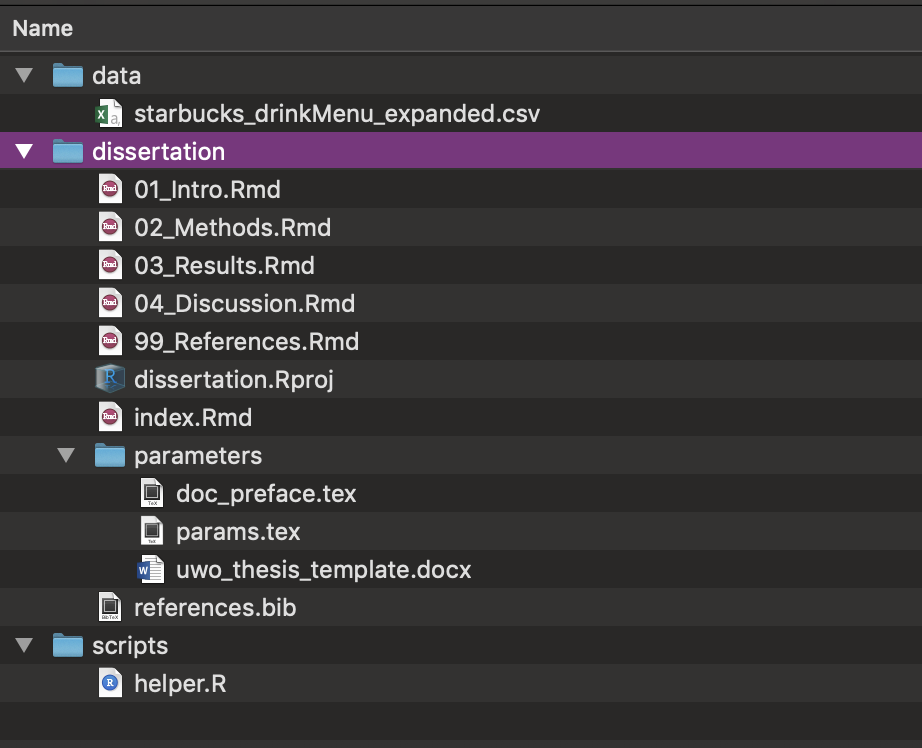
\includegraphics{images/dir_structure.png}

In this example\ldots{}

\textbf{dissertation} contains your individual RMarkdown files that contain the bulk of the text of the dissertation.

\begin{itemize}
\item
  \texttt{index.Rmd}: Contains your YAML that will tell bookdown how to render your book
\item
  \texttt{.Rmd} files that comprise the body of your book. These can be specific chapters, but can also be constructed modularly in whatever way you choose.

  \begin{itemize}
  \tightlist
  \item
    Unless specifically told otherwise, bookdown will compile these in \emph{alphanumeric order}, so they should be named in the order you want them to appear.
  \item
    In a nutshell, file names should be \textbf{machine readable, human readable, and play well with default ordering} \href{https://speakerdeck.com/jennybc/how-to-name-files}{(thank you, Jenny Bryan)}.
  \item
    The names of the files themselves don't appear anywhere in the final document. For that, you need to use headers within the body of the .Rmd documents
  \end{itemize}
\item
  \texttt{references.bib} is a bib file containing your references. Most popular reference management tools have the option to export your references to a .bib file.
\item
  \texttt{parameters} contains the files necessary to tell \texttt{bookdown} how to render your final document.

  \begin{itemize}
  \tightlist
  \item
    If you are compiling to a \textbf{PDF}, it needs 2 .tex (Latex) files: \texttt{doc\_preface.tex}, which contains the ``front matter'' of your dissertation (acknowledgements, etc), and \texttt{params.tex}, which contains the Latex parameters required to compile
  \item
    If you are compiling to a \textbf{Word document}, it needs a template file. This could technically just be a blank document. The important thing is that it has been saved with the Word styles you want to employ in your final .docx output.
  \end{itemize}
\end{itemize}

\textbf{data} contains any raw data files (.csv, .xlsx, etc.). Ideally, these don't get touched after you put them here, because any further manipulation will be done using .R scripts (which will make it easier to track your changes to the data)

\textbf{scripts} contains any helper scripts you used along the way (e.g., for your analysis)

\textbf{More resources:}

\begin{itemize}
\tightlist
\item
  \href{https://swcarpentry.github.io/r-novice-gapminder/02-project-intro/}{Software Carpentry's guide on project management in R Studio}
\item
  \href{https://twitter.com/CivicAngela/status/1024469727274565633}{Angela Li's thread on thesis structuring}
\end{itemize}

\hypertarget{writing-a-chapter}{%
\section{Writing a chapter}\label{writing-a-chapter}}

We will now create a single chapter in RMarkdown.

There is a \emph{lite} and a \emph{heavy duty} version of this.

The lite version will help us learn:

\begin{itemize}
\tightlist
\item
  the minimal components of a \texttt{bookdown} chapter
\end{itemize}

\textbf{Go to the lite version in exercise 2 in Section \ref{ex2}}

The heavy-duty version will help us learn how to incorporate:

\begin{itemize}
\tightlist
\item
  data
\item
  helper .R script
\item
  citations
\item
  figures/tables
\end{itemize}

\textbf{Go to the heavy-duty version in exercise 3 in Section \ref{ex3}}

\hypertarget{making-a-book}{%
\section{Making a book!}\label{making-a-book}}

Now that we have the bare bones of a dissertation, we can compile it for the first time.

Recall that, for this method, the \textbf{essential ingredients} are:

\begin{itemize}
\tightlist
\item
  your .Rmd files (chapters)
\item
  index.Rmd
\end{itemize}

\textbf{Optional ingredients:}

\begin{itemize}
\tightlist
\item
  references.bib
\item
  templates
\end{itemize}

\hypertarget{the-workhorses}{%
\subsection{The workhorses}\label{the-workhorses}}

The files that will do the heavy lifting in order for your dissertation to compile are:

\begin{itemize}
\tightlist
\item
  \texttt{index.Rmd} contains the YAML\footnote{\href{https://en.wikipedia.org/wiki/YAML}{YAML} (rhymes with camel): The header that tells R Markdown how to generate your document. Indentation and spacing are very important. Stands for}
\end{itemize}

\hypertarget{intermediary-stages}{%
\subsection{4. Intermediary stages}\label{intermediary-stages}}

\begin{itemize}
\tightlist
\item
  Previews (with bookdown, or just with Rmarkdown)
\end{itemize}

\hypertarget{the-nitty-gritty}{%
\subsection{5. The nitty gritty}\label{the-nitty-gritty}}

In descending order of messiness (i.e., how confused I get{[}\^{}2{]})

\begin{itemize}
\tightlist
\item
  Reference management + citations
\item
  Notes to self within text
\item
  Snippets! 💕
\item
  Predefined functions
\item
  Footnotes
\item
  Cross-referencing sections/figs/tables
\item
  Figure/table autonumbering
\item
  Tables in RMarkdown

  \begin{itemize}
  \tightlist
  \item
    Specifically when working with both .docx and .pdf
  \end{itemize}
\item
  Appendices
\end{itemize}

\hypertarget{lets-start-dissertating-with-a-.docx-output}{%
\section{Let's start dissertating with a .docx output}\label{lets-start-dissertating-with-a-.docx-output}}

\hypertarget{template}{%
\subsection{Template}\label{template}}

\begin{itemize}
\tightlist
\item
  Western has a .docx thesis template. This includes detailed descriptions of what should go in the final document, but importantly for our purposes here, all we need are the \emph{styles} specified within this document.

  \begin{itemize}
  \tightlist
  \item
    This could technically just be a blank document. We use it to tell RMarkdown\footnote{Well, really to tell RMarkdown what to tell Pandoc\ldots{}} how to style the final output in Word
  \item
    See also \texttt{custom\_template.docx} from previous \href{LINK}{RMarkdown workshop} to see what I mean
  \end{itemize}
\end{itemize}

\hypertarget{other-resources}{%
\section{Other resources}\label{other-resources}}

\begin{itemize}
\tightlist
\item
  Other Rmd + bookdown resources
\end{itemize}

\hypertarget{dissertating-in-bookdown}{%
\section{Dissertating in Bookdown}\label{dissertating-in-bookdown}}

\hypertarget{essential-ingredients}{%
\subsection{Essential ingredients}\label{essential-ingredients}}

\begin{itemize}
\tightlist
\item
  \texttt{index.Rmd}: Contains your YAML that will tell bookdown how to render your book
\item
  \texttt{.Rmd} files that comprise the body of your book. These can be specific chapters, but can also be constructed modularly in whatever way you choose.

  \begin{itemize}
  \tightlist
  \item
    Unless specifically told otherwise, bookdown will compile these in \emph{alphanumeric order}, so they should be named in the order you want them to appear.

    \begin{itemize}
    \tightlist
    \item
      In a nutshell, file names should be \textbf{machine readable, human readable, and play well with default ordering} \href{https://speakerdeck.com/jennybc/how-to-name-files}{(thank you, Jenny Bryan)}.
    \end{itemize}
  \end{itemize}
\end{itemize}

\hypertarget{non-essential-but-very-helpful-ingredients}{%
\subsection{Non-essential but very helpful ingredients}\label{non-essential-but-very-helpful-ingredients}}

\begin{itemize}
\tightlist
\item
  A \texttt{.bib} file contianing your references
\item
  Separate directories containing your:

  \begin{itemize}
  \tightlist
  \item
    data (raw .csv files, etc)
  \item
    scripts (helper \texttt{.R} scripts that contain the bulk work of your analyses)
  \item
    images that are not created in R
  \end{itemize}
\item
  \textbf{Template documents} that will provide bookdown with the information it needs to style your document

  \begin{itemize}
  \tightlist
  \item
    \textbf{Word}: \texttt{uwo\_thesis\_template.docx} is a Word document containing the style settings required to output a Western-approved thesis. This template also contains text, but really all you need is a Word document with the style elements set that you wish to use
  \item
    \textbf{PDF}: The \texttt{tex} folder contains two \texttt{.tex} files that use Latex to create a final PDF:

    \begin{itemize}
    \tightlist
    \item
      \texttt{params.tex} contains the Latex parameters required to compile the document
    \item
      \texttt{doc\_preface.tex} contains the \emph{front matter}: everything that will appear before the beginning of the thesis
    \end{itemize}
  \end{itemize}
\end{itemize}

\emph{A note on the .tex documents:} The documents provided here are comprised of a mash-up of two extremely useful resources:

\begin{itemize}
\tightlist
\item
  \href{https://livefreeordichotomize.com/2018/09/14/one-year-to-dissertate/}{Lucy D'Agostino McGowan's blogpost and dissertation toolkit} provided the original versions of these documents and a super handy walkthrough on how to use them.
\item
  \href{https://github.com/jclauneuro/thesis_template}{Jon Clau's updated Western .tex templates} contain the information necessary to produce a Western U thesis (the files hosted on \href{https://grad.uwo.ca/academics/thesis/formatting.html}{Western's site} are older versions)
\end{itemize}

\hypertarget{rendering-the-book}{%
\subsection{Rendering the book}\label{rendering-the-book}}

Once you have more than one \texttt{.Rmd} file, you are ready to render/compile them into a fully combined document.

The rendered version will appear in \texttt{\_book/}

To render the book as whatever is listed as the default in \texttt{index.Rmd}, do:

\begin{verbatim}
bookdown::render_book("index.Rmd")
\end{verbatim}

To render as a pdf or word document, do:

\begin{verbatim}
bookdown::render_book("index.Rmd", output_format = "pdf_book")
bookdown::render_book("index.Rmd", output_format = "word_document2")
\end{verbatim}

A nice way to preview it is to render it as a gitbook:

\begin{verbatim}
bookdown::render_book("index.Rmd", "bookdown::gitbook")
\end{verbatim}

Then open index.html in your browser, and run \texttt{bookdown::serve\_site()} to update it whenever you save changes. This is much neater/navigable.

Beware of features that will only show up in pdf rendering (like certain features of kable, kableExtra), or that won't compile for pdfs (like the emo package)

\hypertarget{exercises}{%
\chapter{Exercises}\label{exercises}}

\hypertarget{ex1}{%
\section{1. Getting started with RMarkdown}\label{ex1}}

\textbf{Make an R Project}

\href{https://support.rstudio.com/hc/en-us/articles/200526207-Using-Projects}{R Projects} make project management really simple. For every new project you embark on, creating a new .RProj file.
Open that .RProj file whenver you're ready to work on that project, and it will:

\begin{itemize}
\tightlist
\item
  Give you easy access to the directory structure (no need to define a working directory)
\item
  Restore your last RStudio session from that project (no need to reopen files)
\item
  Give you access to your R history from your last session
\item
  \emph{NB: these preferences can all be tweaked}
\end{itemize}

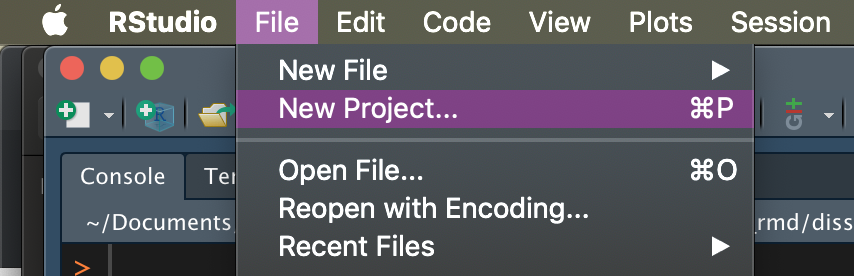
\includegraphics{../images/new_project.png}

\begin{itemize}
\tightlist
\item
  Follow the prompts to create a project in a new directory for this workshop
\end{itemize}

\textbf{Make a new .Rmd file}

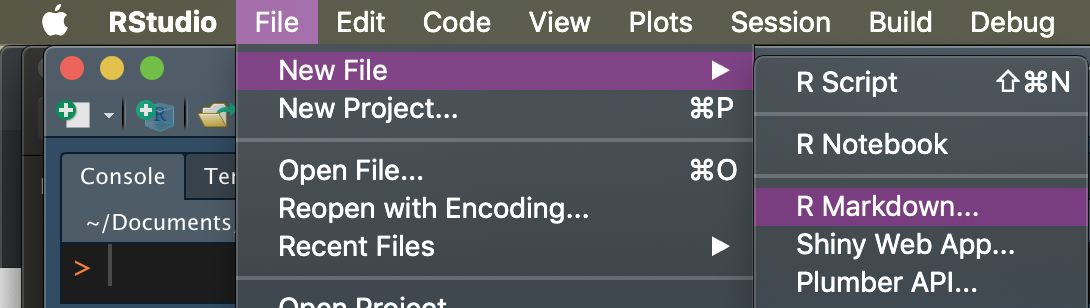
\includegraphics{../images/new_rmd.png}

These are the components of your RMarkdown file:

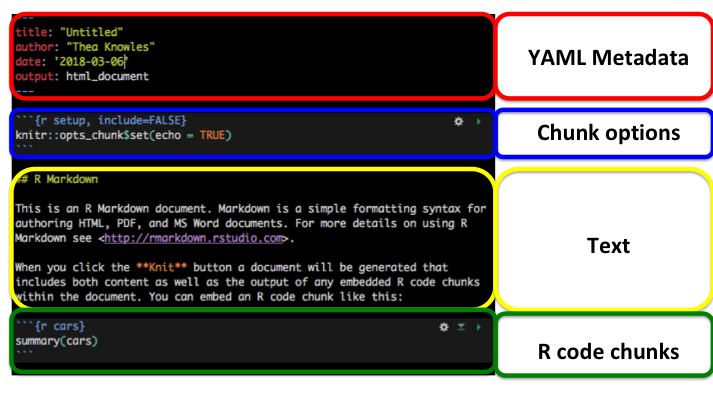
\includegraphics{images/rmarkdown_parts.png}

We won't go into this in \emph{too} much detail

\textbf{Knit your document}

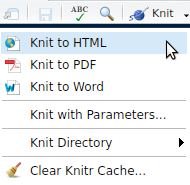
\includegraphics{images/knit.png}

Try it as a\ldots{}

\begin{itemize}
\tightlist
\item
  Word document
\item
  Html document
\item
  PDF document
\end{itemize}

\textbf{More resources}

\begin{itemize}
\tightlist
\item
  \href{https://rmarkdown.rstudio.com/lesson-1.html}{RStudio intro to RMarkdown}
\item
  R-Ladies \#LdnOnt presentations

  \begin{itemize}
  \tightlist
  \item
    \href{https://github.com/rladies/meetup-presentations_london_ontario/tree/master/2017-03-04_Intro2RMarkdown}{Intro to RMarkdown}
  \item
    \href{https://github.com/rladies/meetup-presentations_london_ontario/tree/master/2018-03-06_rmarkdown}{RMarkdown for summary reports and journal articles} (also see more specific resources on the last slide)
  \end{itemize}
\end{itemize}

Back to Section \ref{rmd-crash-course}

\hypertarget{ex2}{%
\section{2. What's in a chapter? Lite version}\label{ex2}}

Open \texttt{01\_Intro.Rmd} and do the following:

\begin{itemize}
\tightlist
\item
  Write some text
\item
  Insert an R chunk that contains some simple R code
\item
  Knit to HTML
\end{itemize}

E.g.,

\begin{Shaded}
\begin{Highlighting}[]
\NormalTok{x =}\StringTok{ }\DecValTok{3}
\NormalTok{x}\OperatorTok{^}\DecValTok{2}
\end{Highlighting}
\end{Shaded}

\begin{verbatim}
## [1] 9
\end{verbatim}

\hypertarget{ex3}{%
\section{3. What's in a chapter? Heavy-duty version}\label{ex3}}

Open \texttt{03a\_Results.Rmd} and find examples of:

\begin{itemize}
\tightlist
\item
  sourcing a helper file (\texttt{helper.R})
\item
  citing references
\item
  generating images and tables from the imported data
\item
  cross-referencing those figures and tables
\item
  using inline R code to refer to values from the data (like p-values, etc) so there's never a need to copy/paste
\end{itemize}

Open \texttt{../scripts/helper.R} to see what it contains.

Open \texttt{03b\_Results.Rmd} and do any of the following:

\begin{itemize}
\tightlist
\item
  source \texttt{helper.R}
\item
  write some text
\item
  cite another source
\item
  make a figure or a table
\item
  Knit the document as an HTML file
\end{itemize}

\textbf{More resources:}
- \href{https://bookdown.org/yihui/bookdown/get-started.html}{Getting started with bookdown}

\hypertarget{explore-.tex-files}{%
\section{4. Explore .tex files}\label{explore-.tex-files}}

\hypertarget{bookdown-to-.pdf}{%
\section{5. Bookdown to .pdf}\label{bookdown-to-.pdf}}

\hypertarget{add-figure}{%
\section{7. Add figure}\label{add-figure}}

\hypertarget{add-table}{%
\section{9. Add table}\label{add-table}}

\hypertarget{edit-refs}{%
\section{10. Edit refs}\label{edit-refs}}

\hypertarget{report-stats}{%
\section{11. Report stats}\label{report-stats}}

\hypertarget{customize-snippets}{%
\section{12. Customize snippets}\label{customize-snippets}}

\hypertarget{results}{%
\chapter{Results}\label{results}}

\hypertarget{limitations}{%
\chapter{Limitations}\label{limitations}}

\emph{I.e., the things I know that I do not yet know}

\hypertarget{other-methods}{%
\section{Other methods}\label{other-methods}}

As mentioned, this is one particular way of doing things. You may also wish to check out R packages people have created for their theses

\begin{itemize}
\tightlist
\item
  \href{https://github.com/ismayc/thesisdown}{thesisdown}: Thesis template designed for Reed College.

  \begin{itemize}
  \tightlist
  \item
    \href{https://thesisdown.netlify.com/}{Gitbook output}
  \item
    \href{https://github.com/ismayc/thesisdown_book/blob/gh-pages/thesis.pdf}{PDF output}
  \end{itemize}
\item
  Many others have developed customized versions of this for their universities. See the \texttt{thesisdown} site for a list of other available templates.
\item
  Perhaps the Western templates could eventually be incorporated in this
\end{itemize}

\hypertarget{woe-is-word}{%
\section{Woe is Word\ldots{}}\label{woe-is-word}}

Many of the issues I run into have to do with strange behaviour in Microsoft Word. For example:

\hypertarget{table-formatting}{%
\subsection{Table formatting}\label{table-formatting}}

Table formatting is ugly with \texttt{kable()}. There are alternatives to \texttt{kable} that are specifically designed for .docx output. These are lovely alternatives to use if you are only outputting to Word (or HTML), but I have repeatedly run into problems with these other options playing nice when alternating between .pdf and .docx outputs.

Table formatting packages for .docx outputs:

\begin{itemize}
\tightlist
\item
  \href{https://cran.r-project.org/web/packages/flextable/vignettes/overview.html}{flextable}
\item
  \href{https://cran.r-project.org/web/packages/captioner/vignettes/using_captioner.html}{captioner}
\item
  \href{https://haozhu233.github.io/kableExtra/save_kable_and_as_image.html}{kableExtra::as\_image()}
\end{itemize}

\hypertarget{references}{%
\chapter{References}\label{references}}

\backmatter
\end{document}
